\section{Mohó algoritmus matroidon és matroid megadása bázissal, duális matroidok}

\[
\begin{rcases}
M=(E,F) \mbox{ matroid}, \\ 
w : E \mapsto \mathbb{R}^+
\end{rcases}
\xRightarrow{?} \parbox[L]{9.8cm}{mekkora a maximális összsulyú független halmaz,
azaz max$\left\{\sum_{e \in X}w(e)\right\}$ ha $X \in F$, és mely ez az $X$?}
\]

\vspace{0.4cm}
\emph{A mohó algoritmus tetszőleges matroid és súlyfüggvényre optimális
megoldást ad a fenti kérdésre, a $\emptyset \in F$--ből kiindulva, maximális
sulyú elemeket csökenő sorrendbe véve (amik nem sértik a halmaz
függetlenségét).}
\vspace{0.4cm}

A bizonyitás indirekt történik, tegyük fel, hogy nem. Legyen ekkor $Y$ az
optimumot meghatározó halmaz, $X$ pedig amit a mohó algoritmus adott. Tudjuk,
hogy $X$ és $Y$ is maximálisan független, tehát az F$3$ alapján $|X|=|Y|=n$. A
két halmaz elemeit rendezzük csökkenő sorrendbe, és írjuk fel őket mint
$X=\{a_1, a_2, \cdots, a_n\}$ és $Y=\{b_1, b_2, \cdots, b_n\}$, ahol:

\begin{align*}
w(a_1) \geq w(a_2) \geq \cdots \geq w(a_n) \\
w(b_1) \geq w(b_2) \geq \cdots \geq w(b_n) \\
\end{align*}

A mohó algoritmus a legnagyobb sulyú elemmet vesszi, amely esetén a
függetlenségi tulajdonság nem sérül, tehát az első elem a legnagyobb elem lesz,
azaz $w(a_1) \geq w(b_1)$. Mivel a két halmaz különböző egymástol, ezért lesz
egy $i$ index amire ez a feltétel megfordul, azaz $ w(b_i)> w(a_i)$, egyébbként
a mohó is az optimumot kapta volna meg. Amely lépésben ez előfordul a két halmaz
felírható mint:

\[
\begin{rcases}
A=\{a_1, \cdots, a_{i-1}\}, \\
B=\{b_1, \cdots, b_{i}\}
\end{rcases} 
\xRightarrow{\mbox{F3}} \exists~b_j \in B, \mbox{ amelyre } A + b_j \in F  
\]

Az $A$ halmaz elemei csökkenő sorrendbe vannak rendezve, tehát $w(b_j) \geq
w(b_i)$, de ugyanakkor itt $w(b_i) > w(a_i)$. De ez ellentmondás, mert ekkor a
mohó algoritmus a $b_j$ elemet választotta volna, nem peddig az $a_i$--t, tehát
feltevéssünk hamis volt, a mohó algoritmus megadja az optimális megoldást.

\vspace{0.4cm}
\emph{Ha a mohó algoritmus optimális megoldást ad és F$1$,F$2$ függetlenségi axiómák
teljesülnek akkor F$3$ is igaz.}
\vspace{0.4cm}

A bizonyitás ismét indirekt, tegyük fel, hogy a mohó algoritmus optimális megoldást ad, de
F$3$ nem lesz igaz. Ilyenkor $X,Y \in F$, ahol $|X|>|Y|$ igaz, de $\not \exists~x \in X-Y$ úgy, hogy
$Y \cup \{x\} \in F$. Legyen:

\[
\begin{rcases}
r=\frac{|Y-X|}{|X-Y|}\\
w : E \mapsto \mathbb{R}^+ \\
w(e) = \begin{cases}
1 & e \in Y, \\
r + \frac{1-r}{2} & e \in X-Y, \\
0 & \mbox{másképp}
\end{cases}
\end{rcases}\Rightarrow
\parbox[L]{8.25cm}{
Az algoritmus elöszőr kiválasztja $Y$ elemeket, de ezután már csak nulla sulyút
választhatna. Így az összsúly ekkor $|Y|\cdot 1$. $X$ összsúly visszont $|X \cap
Y| + |X-Y|\cdot(r+\frac{1-r}{2})$, ami nagyobb. De így egy optimálisabb megoldást
kaptunk, azaz a mohó nem az optimumot adta meg. De ez elentmond a kiinduló feltételünknek,
tehát a feltvésünk, hogy $F$3 nem teljesül, hamis. } \]

\begin{figure}[htbp]
\centering
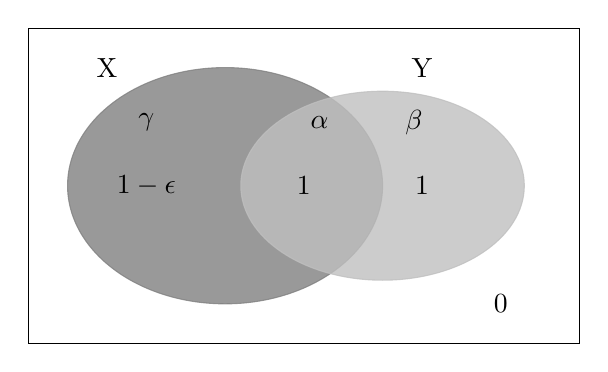
\begin{tikzpicture}
	\draw  (-1.5cm,1.5cm) node{X};
	\draw  (2.5cm,1.5cm) node{Y};
	\draw  (3.5cm,-1.5cm) node{$0$};
	\draw  (4.5cm,-2cm) rectangle (-2.5cm,2cm);
	\begin{scope}[opacity=0.8]
		\filldraw[fill=gray, draw=gray] (0,0) ellipse (2cm and 1.5cm) ;
		\filldraw[fill=lightgray, draw=lightgray] (2cm,0) ellipse (1.8cm and 1.2cm) ;
	\end{scope}
	\draw  (-1cm, 0) node[color=black]{$1-\epsilon$};
	\draw  (1cm, 0) node[color=black]{$1$};
	\draw  (2.5cm, 0) node[color=black]{$1$};
	\draw  (-1.0cm,0.8cm) node{$\gamma$};
	\draw  (1.2cm,0.8cm) node{$\alpha$};
	\draw  (2.4cm,0.8cm) node{$\beta$};
\end{tikzpicture}
\caption{Ha a mohó algoritmus megoldása optimális, akkor F3 teljesül}\label{fig:Mohó}
\end{figure}

\subsection{Bázisos megadás}
Legyen $B$ egy matroid bázisainak halmaza, ekkor teljesül, hogy:

\[
\begin{cases}
\mbox{B1)} & B \neq \emptyset \\
\mbox{B2)} & |X_1|=|X_2| \Leftarrow \forall X_1,X_2 \in B\\
\mbox{B3)} & \begin{rcases}
X_1, X_2 \in B \\
e_1 \in X_1
\end{rcases}\Rightarrow \exists~e_2 \in X_2, \mbox{hogy } X_1-e_1+e_2 \in B \\
\end{cases}
\]

Fordítva, ha $(E,B)$ egy halmazrendszer ahol a fenti három tulajdonság teljesül akkor $M=(E,F)$
matroidot alkot, ahol:

\[
F = \left\{H: H \subseteq C \mbox{ valamely } C \in B\mbox{--re}\right\}
\]

\subsection{Duális matroid}

\[
\begin{rcases}
M=(E,F) \mbox{ matroid}, \\
\mbox{bázisai } B=\{B_1, \cdots, B_n\}
\end{rcases} \Rightarrow
\parbox[L]{9cm} {
A duális matroid bázisai megfogalmazható mint $B^*=\{E-B_1, \cdots, E-B_n\}$.
Ez meghatározza $F^*$--ot, és duális matroidot mint $M^*=(E,F^*)$ jelöljük.}
\]

Bizonyitanunk kell, hogy az $M^*$ matroidra teljesülnek a függetlenségi axiómák.
F$1$ és F$2$ nyilvánvaló. F$3$--at kell belátni, azaz, hogy $X,Y \in F^*$ és
$|X|>|Y|$ esetébben létezzik $x \in X-Y$, hogy $Y+x \in F^*$. Legyen $B_X
\subseteq E-X$ és $B_Y\subseteq E-Y$ egy--egy $M$--beli bázis, amelyek a
definició alpaján léteznek.

Ha létezzik $X$--beli elem amely nincs benne $Y$--ban és $B_Y$--ban se, akkor
ezt hozzávéve $Y$--hoz ismét $F^*$--beli halmazt kapnánk. Ha ilyen nem létezzik akkor 
$X \subseteq B_Y \cup Y$ és

\[
|B_Y \cap X | = |X-(X \cap Y)| > |Y - (X \cap Y)| \geq |B_X \cap Y|.
\]

$B_X$ és $B_Y$ mérete megegyezik ($|B_X|=|B_Y|$), tehát $|B_Y-X| < |B_X-Y|$.
Most e két halmazra alkalmazzuk F$3$--at, azaz $\exists~z \in (B_X-Y)-(B_Y-X)$
eleme amelyre $(B_Y-X)+z$ független $M$--ben. Ezt a független halmazt egészitsük
ki bázisá, úgy, hogy $B_Y$--ból vesszünk hozzá új elemeket, jelöljük ezt
$B'$--el. $B'$ bázisába létezik elem $E-B_Y$--ból, tehát létezik olyan $B_Y$--beli elem 
amely nincs benne $B'$--ben. Legyen ez az elem $u$. E $u$ elemre $Y+u \subseteq E - B'$,
tehát $Y+u \in F^*$. Megkaptuk az elemet amire mindig igaz lesz F$3$, tehát a bizonyitás
teljes. 

\[(M^*)^* = M \]

\subsection{A duális matroid rangfüggvénye}

\[ r^*(X) = |X|-r(E)+r(E-X)\]

A bizonyitáshoz csupán le kell vezetni:

\begin{align*}
r^*(X) &= \mbox{max} \{ |X \cap Y| : Y \in F^*\}   = \mbox{max} \{ |X \cap Y| : Y \in B^*\}\\
       &= \mbox{max} \{ |X \cap (E-Z)| : Z \in B\} = |X| - \mbox{min} \{ |Z \cap X| : Z \in B\}\\
       &= |X| - (r(E)-\mbox{max}\{|W \cap (E-X)| : W \in B\}) \\
       &= |X| - r(E) + r(E-X)
\end{align*}